\section{Title}
Engineering problems are mostly viewed as the approximation problems, in which people try to find the possible solutions as near to the true solutions as possible and the optimization process involves to minimize the misfit function. The inversion problem regarded as a very complex problem to solve deals with uncertainty and non-uniqueness of solutions. The search on applying geophysical techniques to explore the geophysical parameters of the ground and then convert them to the geotechnical parameters for civil engineering application is large. 


\begin{table}[h!]
    \centering
    \caption{Caption}
    \begin{tabu}{*{4}{X[c]}}
        \toprule
            \textbf{Name} & \textbf{Age} & \textbf{Height} & \textbf{Width} \\
        \midrule
            Cater & 20 & 68 & 90 \\
            Andy & 20 & 68 & 90 \\
            Peter & 20 & 68 & 90 \\
        \bottomrule
    \end{tabu}
    \label{tab:table}
\end{table}


\section{Title}
However, the process of inversion is complicated dealing with various parameters and the uncertainty of the data caused by field conditions and human performance. One example is the dispersion of wave propagation in soil medium, there is not only one mode phase velocity dispersion curve, but multiple modes. 

\begin{figure}[!t]
    \centering
    \begin{subfigure}[b]{0.3\textwidth}
        \centering
        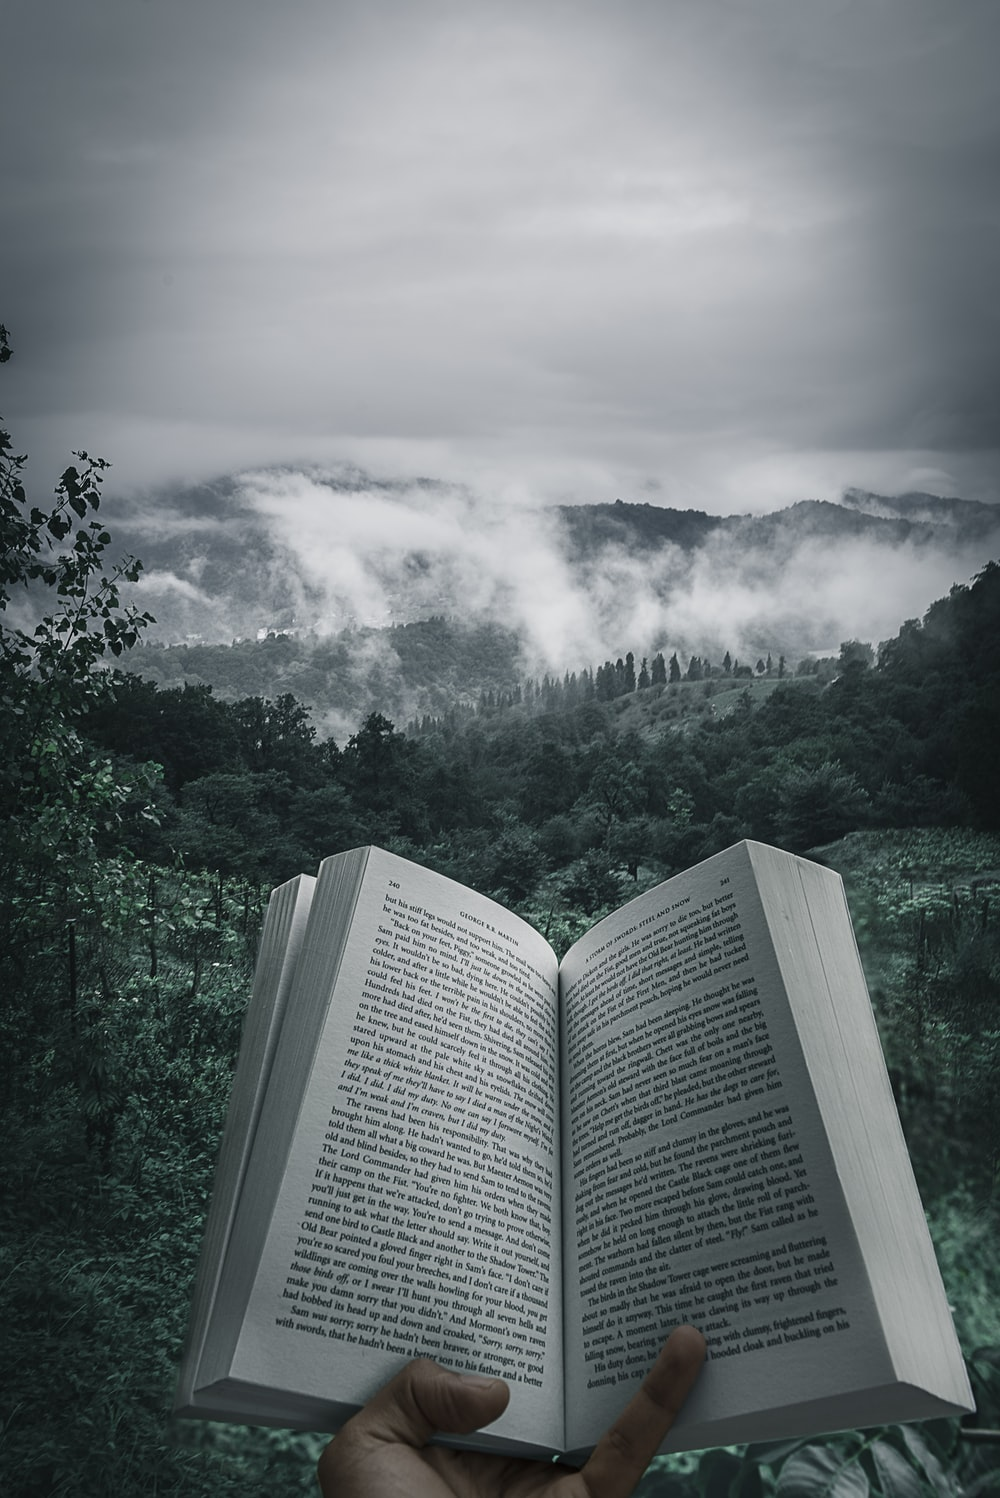
\includegraphics[width=\textwidth]{images/f}
        \caption{$y=$x}
        \label{fig:wave1}
    \end{subfigure}
    \hfill
    \begin{subfigure}[b]{0.3\textwidth}
        \centering
        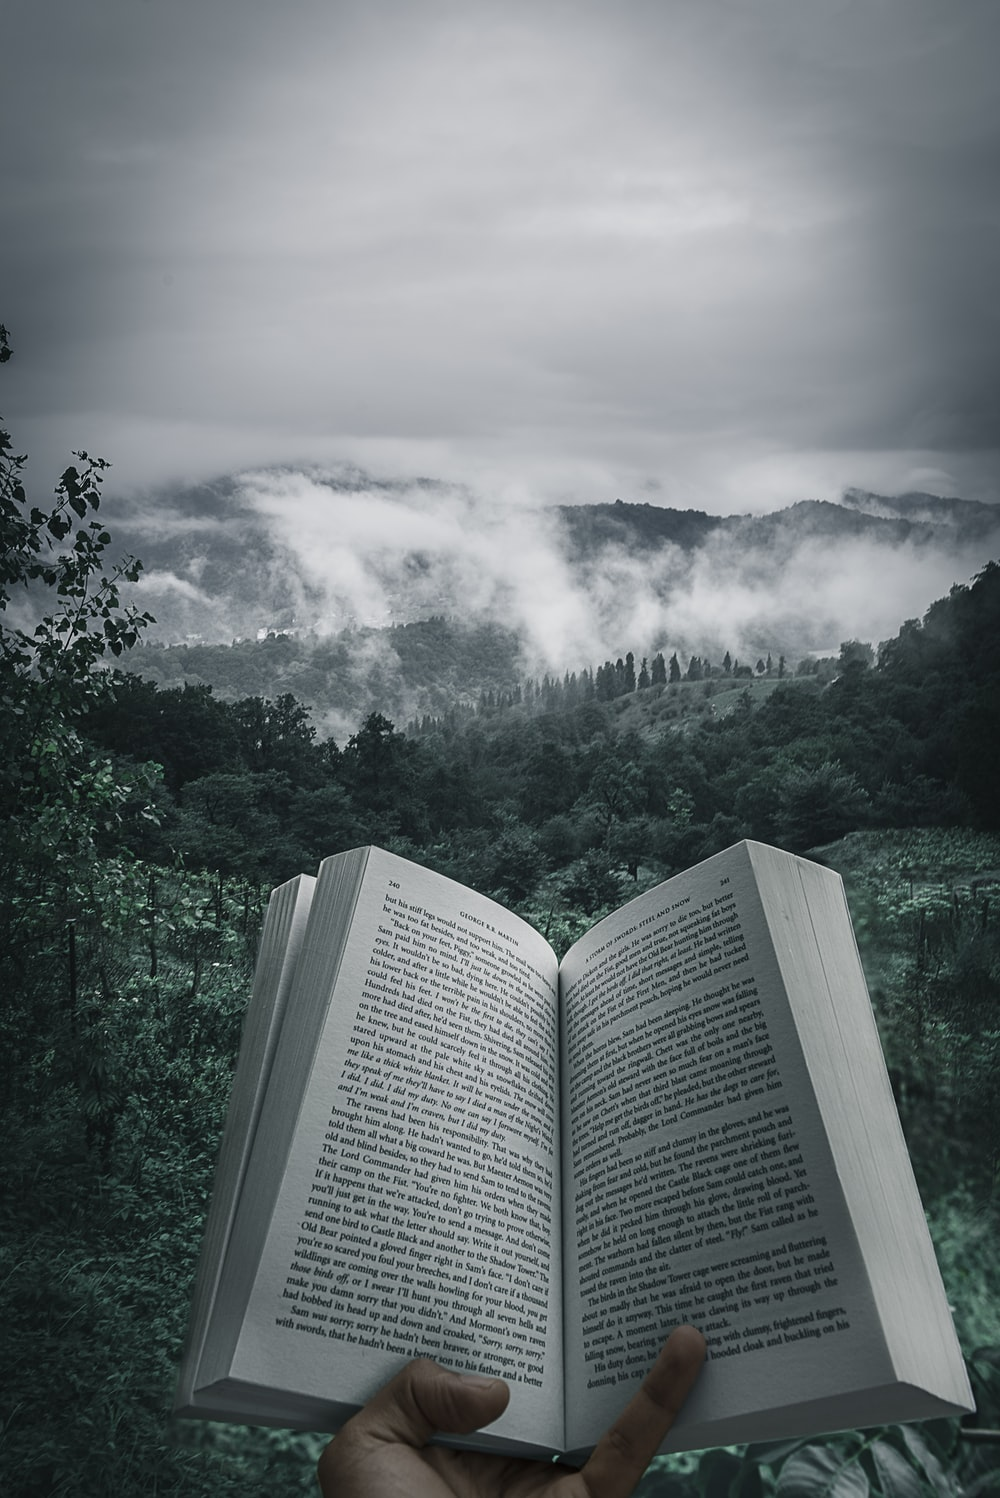
\includegraphics[width=\textwidth]{images/f}
        \caption{$y=$x}
        \label{fig:wave1}
    \end{subfigure}
    \hfill
    \begin{subfigure}[b]{0.3\textwidth}
        \centering
        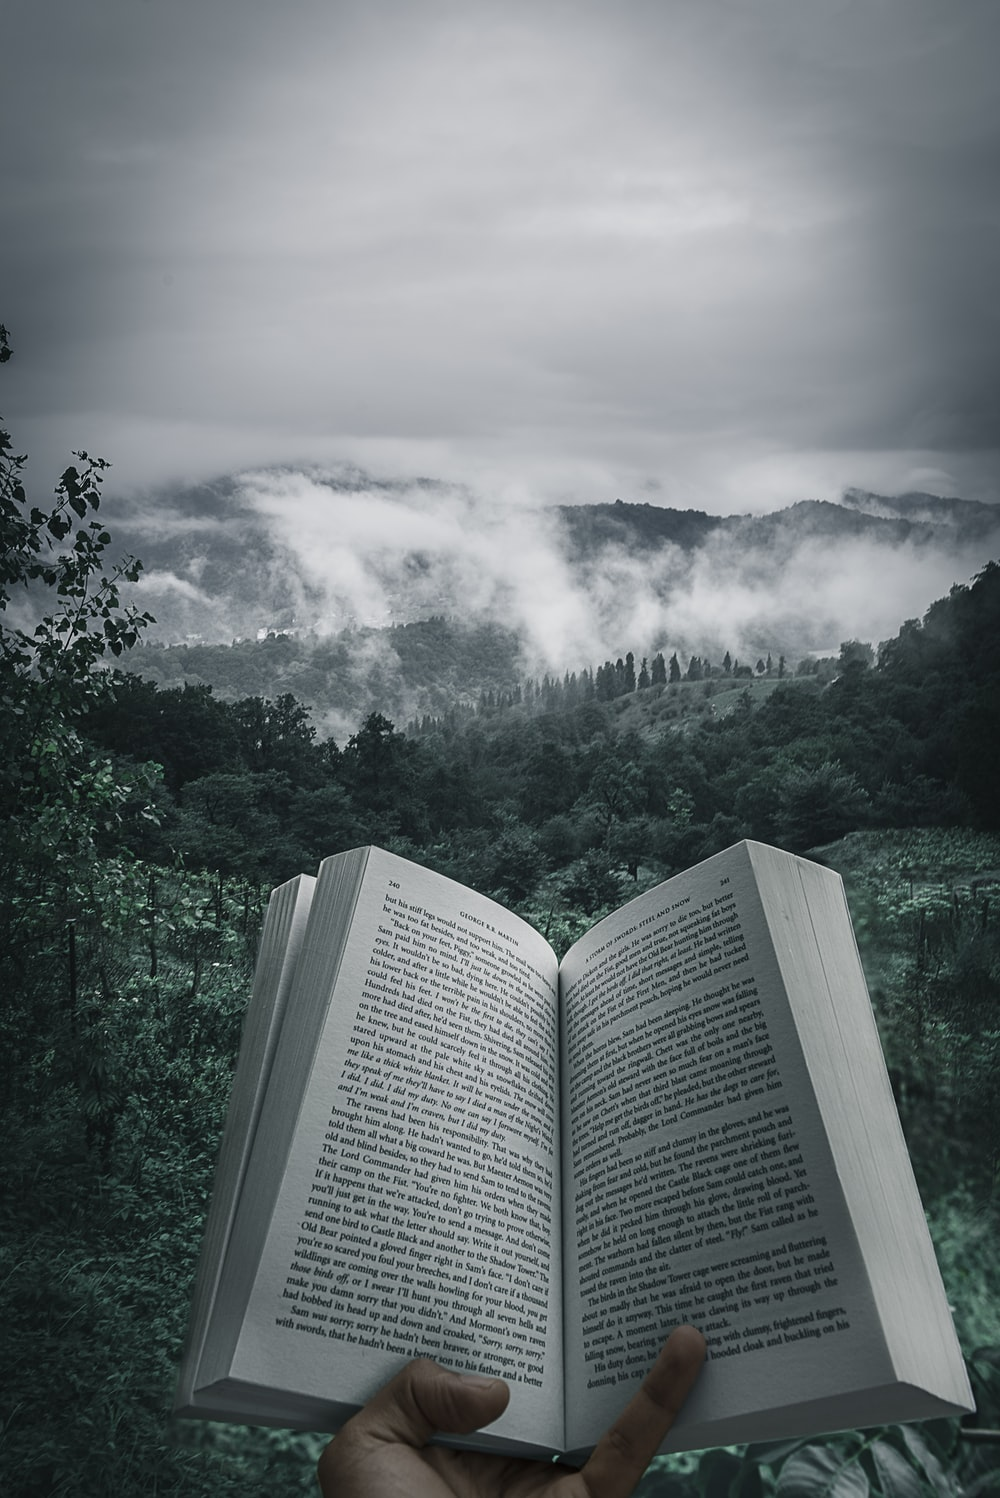
\includegraphics[width=\textwidth]{images/f}
        \caption{$y=$x}
        \label{fig:wave1}
    \end{subfigure}
    \hfill
    \caption{Waves}
    \label{fig:three waves}
\end{figure}    

The picking approach of dispersion curve has been considered to be highly objective, different people pick in different manner. The automated inversion algorithms are widely applied, but also very dangerous because of the complicated occurrence of higher-order modes and the argument of garbage in, garbage out.

\begin{figure}[!t]
    \centering
    \begin{subfigure}[b]{0.45\textwidth}
        \centering
        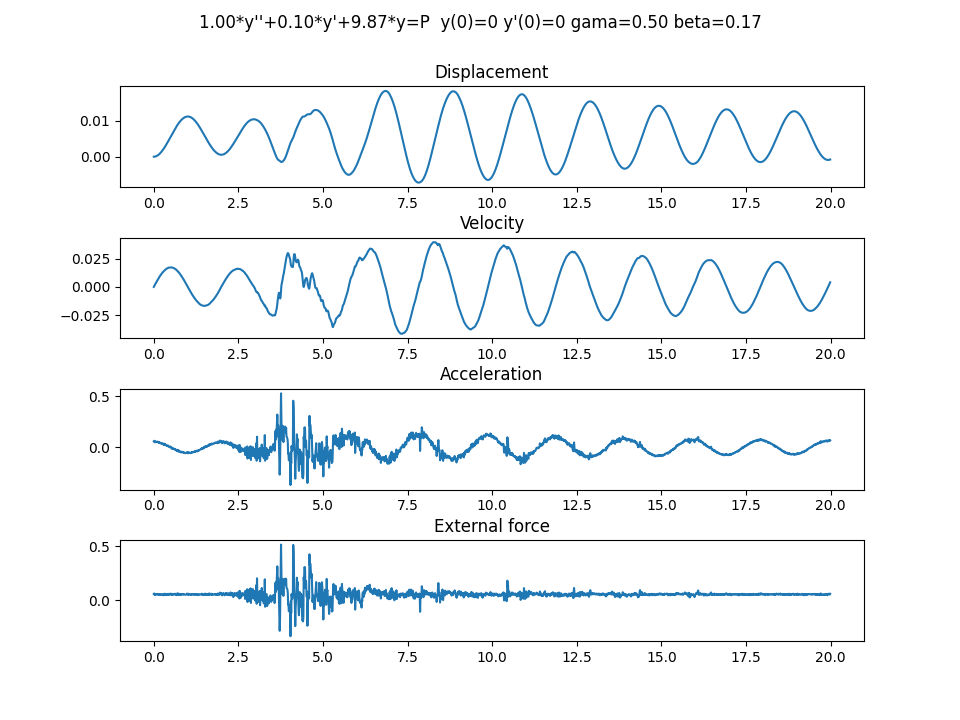
\includegraphics[width=\textwidth]{images/f1.png}
        \caption{Figure}
        \label{tab:wave1}
    \end{subfigure}
    \hfill
    \begin{subfigure}[b]{0.45\textwidth}
        \centering
        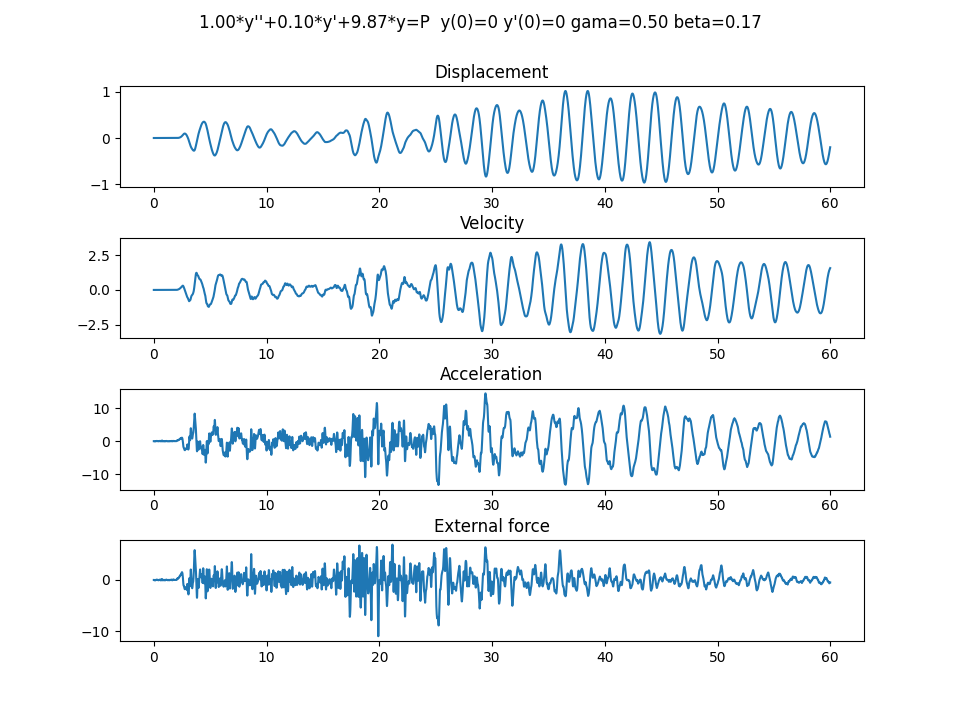
\includegraphics[width=\textwidth]{images/f2.png}
        \caption{}
        \label{tab:wave2}
    \end{subfigure}
    \hspace{1em}
    \caption{Figure}
    \label{tab:wave}
\end{figure}

\section{Title}
The picking approach of dispersion curve has been considered to be highly objective, different people pick in different manner. The automated inversion algorithms are widely applied, but also very dangerous because of the complicated occurrence of higher-order modes and the argument of garbage in, garbage out.


\begin{figure}[!t]
    \centering
    \begin{subfigure}[b]{0.45\textwidth}
        \centering
        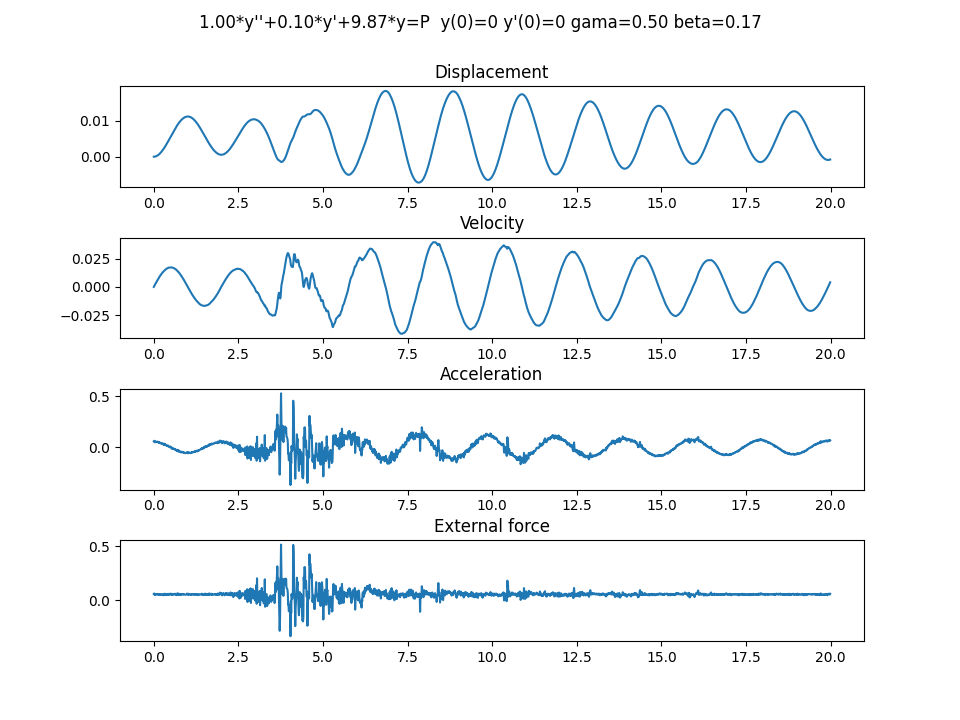
\includegraphics[width=\textwidth]{images/f1.png}
        \caption{Figure}
        \label{tab:wave1}
    \end{subfigure}
    \hfill
    \begin{subfigure}[b]{0.45\textwidth}
        \centering
        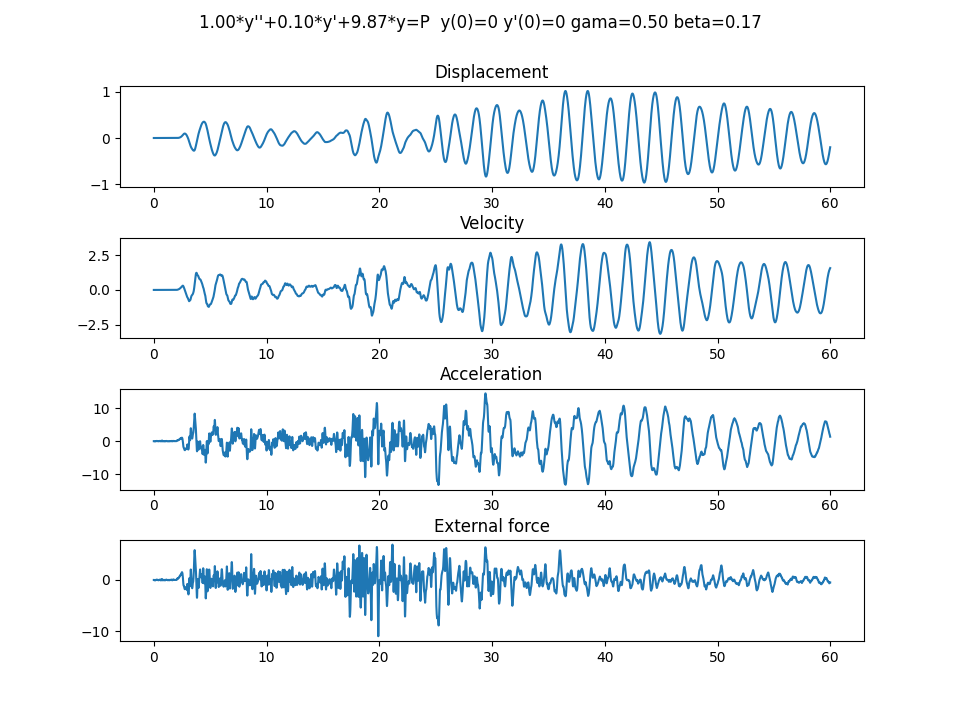
\includegraphics[width=\textwidth]{images/f2.png}
        \caption{}
        \label{tab:wave2}
    \end{subfigure}
    \hspace{1em}
    \caption{Figure}
    \label{tab:wave}
\end{figure}
